% !TEX options=--shell-escape

\documentclass[a4paper,10pt,openright]{memoir}

\setlength{\parindent}{0mm}

% Style of front page, title page, and stuff page
\usepackage{dikuReport}

% Not resetting figure counter on chapter
\usepackage{chngcntr}
\counterwithout{figure}{chapter}
\renewcommand\thefigure{\arabic{figure}}


% Packages
\usepackage{listings}
\usepackage{minted}      % Syntax highlighting
\usepackage[all]{xy}
\usepackage{eucal}
\usepackage{enumerate}
\usepackage{hyperref}
\usepackage{wrapfig} % side captions on figures
\usepackage[justification=centering]{caption}
\usepackage{url}
\usepackage{mathptmx}
\usepackage{tabularx,colortbl}
\usepackage[normalem]{ulem}
\usepackage{soul}
\usepackage{eso-pic} % \AddToShipoutPicture
\usepackage{fancyhdr}
\usepackage{moreverb}
\usepackage{lscape}
\usepackage[stable]{footmisc}
\usepackage[latin1, utf8]{inputenc}
\usepackage{latexsym}
\usepackage[T1]{fontenc}
\usepackage{cite}
\usepackage{pdfpages}
\usepackage{tikz}
\usepackage{fix-cm}
\usepackage{xcolor,calc, colortbl}
\usepackage{graphicx}
\usepackage{amsbsy}
\usepackage{amsfonts}
\usepackage{amssymb}
\usepackage{amsmath}
\usepackage{alltt}
\usepackage{float}
\usepackage{color}
\usepackage{relsize}
\usepackage{calc}
\usepackage{ifthen}
\usepackage{xspace}
\usepackage{caption}
\usepackage{lipsum}
\usepackage{listings}
\usepackage{color}
\usepackage{multicol}
\usepackage{xparse} % newDocumentCommand
\usepackage{enumitem}
\usepackage{csquotes}

% Color tabulars

\newcommand{\mc}[2]{\multicolumn{#1}{c}{#2}}
\definecolor{Gray}{gray}{0.85}
\definecolor{LightCyan}{rgb}{0.88,1,1}
\newcolumntype{a}{>{\columncolor{Gray}}c}
\newcolumntype{b}{>{\columncolor{white}}c}

% Shorts for sc and bf
\renewcommand{\sc}{\textsc}
\renewcommand{\bf}{\textbf}

%%%%% Make abbreviations emphasized.
\newcommand{\ie}{\emph{i.e.}\xspace}
\newcommand{\eg}{\emph{e.g.}\xspace}
\newcommand{\etc}{\emph{etc.}\xspace}
\newcommand{\vs}{\emph{vs.}\xspace}
\newcommand{\cf}{\emph{cf.}\xspace}
\newcommand{\viz}{\emph{viz.}\xspace}
\newcommand{\etal}{\emph{et~al.}\xspace}

%%% theorem commands
\newtheorem{definition}{Definition}[section]
\newtheorem{theorem}{Theorem}[section]

% Include some layout setup.
%!TEX root = main.tex

% NO RESETTING OF FOOTNOTES AT CHAPTER CHANGE
\usepackage{remreset}
\makeatletter\@removefromreset{footnote}{chapter}\makeatother

% Set the style of chapter heads

%\definecolor{TemplateColor}{rgb}{.75,.116,.60}  % KU Red
\definecolor{TemplateColor}{rgb}{.2941,.4549,.2359} % KU green

\newcommand{\pnumb}[1]{
    \begin{tikzpicture}
      \draw[fill,color=gray] (0,0) rectangle (5mm,5mm);
      \draw[color=white] (2.5mm,2.5mm) node { #1};
    \end{tikzpicture}
}    
\newcommand{\printchapternumm}{}
\makechapterstyle{combined}{
  \setlength{\midchapskip}{-60pt}
  \setlength{\afterchapskip}{2.5cm}
  \setlength{\parskip}{5mm}
  \renewcommand*{\printchaptername}{}
  \renewcommand*{\chapnumfont}{\normalfont\bfseries\fontsize{45}{0}\selectfont}
  \renewcommand*{\printchapternum}{\flushright\chapnumfont\textcolor{TemplateColor}{\thechapter}}
  \renewcommand*{\chaptitlefont}{\normalfont\Huge\bfseries}
  \renewcommand*{\printchaptertitle}[1]{%
    \raggedright\chaptitlefont\parbox[t]{\textwidth-2cm}{\raggedright##1}}
}

% Normal page numbering layout. How is always looks
\newcommand{\normalPN}{\makeevenfoot{plain}{}{\hspace{2mm}\thepage}{}\makeoddfoot{plain}{}{\thepage}{}}

% Special page numbering layout that is used for papers. Numbers are written in a gray box.
\newcommand{\specialPN}{\makeevenfoot{plain}{}{\\~\\~\\\hspace{2mm}\pnumb{\thepage}}{}\makeoddfoot{plain}{}{\\~\\~\\\pnumb{\thepage}}{}}

% Only clearpage (not cleardoublepage) at new chapter.
\renewcommand{\clearforchapter}{\clearpage}

\definecolor{codegreen}{rgb}{0,0.6,0}
\definecolor{codegray}{rgb}{0.5,0.5,0.5}
\definecolor{codepurple}{rgb}{0.58,0,0.82}
\definecolor{backcolour}{rgb}{0.95,0.95,0.92}
\captionsetup{labelfont=bf}

% Custom listing environment
\lstdefinestyle{mystyle}{
    backgroundcolor=\color{backcolour},   
    commentstyle=\color{codegreen},
    keywordstyle=\color{magenta},
    numberstyle=\tiny\color{codegray},
    stringstyle=\color{codepurple},
    basicstyle=\footnotesize,
    breakatwhitespace=false,         
    breaklines=true,                 
    captionpos=b,                    
    keepspaces=true,                 
    numbers=left,                    
    numbersep=5pt,                  
    showspaces=false,                
    showstringspaces=false,
    showtabs=false,                  
    tabsize=2
}

\lstdefinelanguage{Hermes}{
  keywords={call, uncall, printf, scanf, u32, u16, u8, true, false, if, for, \%u32},
  keywordstyle=\color{blue}\bfseries,
  ndkeywords={class, export, boolean, throw, implements, import, this},
  ndkeywordstyle=\color{darkgray}\bfseries,
  identifierstyle=\color{black},
  sensitive=false,
  comment=[l]{//},
  morecomment=[s]{/*}{*/},
  commentstyle=\color{codegreen}\ttfamily,
  stringstyle=\color{red}\ttfamily,
  morestring=[b]',
  morestring=[b]"
}

\lstdefinelanguage{mosml}{
  keywords={let, val, if, then, else, in, end, case, of, fun},
  keywordstyle=\color{blue}\bfseries,
  ndkeywords={HERMES, RSSA, ARM, Var, Update, Array, Assign, For, Const, Block, COMMENT, MOV, ROL, ADD, LDR, STR, SUB, MUL, DIV},
  ndkeywordstyle=\color{darkgray}\bfseries,
  identifierstyle=\color{black},
  sensitive=false,
  comment=[l]{//},
  morecomment=[s]{/*}{*/},
  commentstyle=\color{codegreen}\ttfamily,
  stringstyle=\color{red}\ttfamily,
  morestring=[b]"
}


\lstset{style=mystyle, aboveskip=20pt,belowskip=20pt, xleftmargin=0.25cm, xrightmargin=0.25cm}

% Sets page numbering layout to normal
%\normalPN

% Where graphic files are located
\graphicspath{{Graphics/}}

% Alters the margins of the pages such that text are _not_ centered. This makes better room for the glue bindings.
\addtolength{\foremargin}{-35pt}
\addtolength{\spinemargin}{15pt}
\checkandfixthelayout

\setcounter{secnumdepth}{2}

% Basic information
\thesistype{Masters Thesis}
\thesiscomment{} % You can leave this blank
\title{Compiling a reversible lightweight cryptography language (Hermes) to assembly language ARM64 with focus on mitigating side-channel vulnerabilities}
\author{Hjalte Abelskov qdp218}
\supervisor{Michael Kirkedal Thomsen }
\date{February 28, 2019} % Hand-in date
%\subject{Mitigating side channel vulnerabilities} % Short abstract not needed.
\begin{document}
\maketitle
\pagenumbering{roman}
\setcounter{page}{3}

% English Abstract
\cleardoublepage
\pagestyle{plain}
\begin{abstract}
This thesis revolves around the reversible programming language Hermes, currently being developed at DIKU as a domain-specific language for implementing symmetric cryptography algorithms on small devices.
The reversibility of Hermes makes us able to give certain guarantees for its safety, in that certain side-channel attacks such as information leakage becomes impossible.
I describe these side-channels as well as reversibility and explain the intention of securing small devices.
I develop a compiler from Hermes to a Reversible Single Static Assignment (RSSA) representation, which could serve as a common ancestor for multiple target assembly languages and help shorten each compilation step to a target assembly language.
I also develop a compiler from RSSA to ARM64 assembly language with abstract register names.
This new implementation gives more control over side-channels as we are no longer dependant on \emph{gcc} and \emph{zerostack}, both of which are being used in the currently existing Hermes to C compiler.
I also implement the 128-bit block cipher algorithm Twofish in Hermes, thereby showing the usefulness of Hermes as a domain-specific language for implementing symmetric cryptographic algorithms.
Finally I compare my Twofish implementation with two reference implementations written in Python and C.

\end{abstract}

% Danish abstract
\clearpage
\begin{resume}
Dette speciale omhandler det reversible programmeringssprog Hermes, der er udviklet på DIKU som et domæne-specifikt sprog med henblik på implementatering af symmetriske krypteringsalgoritmer på små enheder.
Reversibiliteten i Hermes gør os i stand til at give nogle garantier for sikkerheden, idet visse side-kanal angreb såsom data-lækage bliver umuliggjort. Jeg beskriver disse side-kanaler samt reversibilitet og forklarer om intentionen om at sikre små enheder.
TODO: Jeg udvikler en ny ?backend? til Hermes, som skal forkorte antallet af trin i oversættelsen til mit valg af arkitektur, som er ARM64. Det vil give mere kontrol over side-kanaler idet vi ikke længere er afhængige af gcc og zerostack som bliver benyttet i den nuværende implementation af Hermes oversættelsen.
Min nye implementation er en to-trins process som først oversætter Hermes til et reversibelt statisk mellemliggende sprog med én tildeling af hver variabel (RSSA), der derfra kan oversættes til diverse arkitekturer - i dette tilfælde ARM64. Denne oversættelse fra RSSA til ARM64 udgør andet trin af oversættelsen.
Jeg implementerer 128-bit block cipheren Twofish og viser derved at Hermes er brugbart som et domæne-specifikt sprog til implementering af symmetriske krypteringsalgoritmer.
TODO: Til slut viser jeg korrektheden ved Twofish implementationen idet jeg anvender et eksisterende bibliotek til property based testing. 
TODO: Consider testing speed of 50 encryptions vs reference solution


\end{resume}

% Table of contents
\setcounter{tocdepth}{1} %Includes section, subsection and subsubsections in TOC
\cleardoublepage
\chapterstyle{combined}
\tableofcontents*

% Starting the real text.
\cleardoublepage
\pagenumbering{arabic}
\setcounter{page}{1}

\chapter{Introduction}
% Huffman, D.A.: Canonical forms for information-lossless finite-state logical machines.IRE Transactions on Information Theory5(5), 41–59 (1959)  First reversible computing guy
%Problemet med sidekanaler (skal lede op til baggrundsafsnittet)
%Nævn evt. også noget om små devices.

% Motivation
For the last hundred years or so, the only way to intercept encrypted messages between parties has been to break the encryption algorithm with crypto analysis. As a result, some very robust cryptography algorithms has been developed that are very hard to attack.
Instead of attacking the algorithm, recent research has focused on vulnerabilities related to the devices that communicate.
It is possible to learn a lot about the data or the algorithm simply from measuring the device on which it resides. Heat generation, time, sound etc. are all components of the cryptograpic event that happened and tell part of the story.
These vulnerabilities are called ``side-channel``-vulnerabilities because they are not directly related to the cryptography algorithms, but rather a byproduct.

And while strong cryptographic methods such as AES (encryption), SHA-256 (hashing) and RSA/Elliptic Curve (signing) work well on systems with reasonable processing power and memory capabilities, they do not scale well into a world with embedded systems and sensor networks.
This introduces some challenges such as how to reduce the amount of costly operations whilst still guaranteeing the highest level of security.
The limits related to physical size, processing power, memory and battery life call for more lightweight cryptography methods to be implemented on such systems.
Lightweight cryptography applications can be implemented in many programming languages, most of which still leave the devices open to side-channels.
The good news is that some of these side-channels are, at least in theory, avoidable if we choose our language of implementation carefully.
One such class of languages are reversible languages, which we will expand on in the following section before coming back to side-channels in Chapter ~\ref{chapt - Side-channel}.

%While conventional cryptography methods, such as AES (encryption), SHA-256 (hashing) and RSA/Elliptic Curve (signing) work well on systems with reasonable processing power and memory capabilities, these do not scale well into a world with embedded systems and sensor networks.
%This introduces some challenges such as how to reduce the amount of costly operations whilst still guaranteeing the highest level of security. The limits related to physical size, processing power, memory and battery life call for more lightweight cryptography methods to be implemented on such systems.
%Lightweight cryptography applications can be implemented in many programming languages, most of which still leave the devices open to more sophisticated hacking methods such as timing attacks.
%These sophisticated hacks exploit weaknesses in physical "side-channels" and are, at least in theory, avoidable if we choose our language of implementation carefully.
%We will expand on reversible computing first, and then come back to side-channels in Chapter ~\ref{chapt - Side-channel}.

\section{Reversible Programming}
% NAND gates are irreversible.
% Landaurs principle is that heat must be generated when doing any "logically irreversible manipulation of information".
Reversible programs can be run both forwards and backwards deterministically, calculating output from input as well as input from output.
What this means is that all functions are bidirectional, i.e. given some resulting output of a function, we can run the inverse of that function with the output and find the initial input.
This is especially useful with algorithms for encryption or encoding, where an inverse process is most often needed.
If implemented without too much overhead, this will result in smaller programs, as the encoding/encryption function is bidirectional and can be used for decoding/decryption as well.

Writing code in a language where all functions are bidirectional imposes some constraints on the programmer: variables local to a function must be initialized as zero and reset to zero after use.
All variable updates must be lossless, therefore not allowing modulo updates such as \lstinline{x = x mod y} as there is no inverse to this operation.
Bit-shift operations must also be lossless, i.e. when bits are rotated off the right end, they are inserted into the vacated bit positions on the left and vice-versa. While imposing some restrictions on the programmer, reversible programming languages has a lot to offer in terms of security: they ensure no loss of information and no variables are left in memory after a program has run, since all variables are reset after use. Thus the memory will not contain any data that can be used for side-channel attacks such as information leakage.

\section{Foundations for this work}
This Master thesis revolves around the reversible programming language Hermes developed at DIKU.
Hermes is based on the reversible programming language Janus and designed specifically for writing encryption algorithms\cite{MogensenHermes}.
By virtue of some carefully thought-out design choices, Hermes offers a built-in protection against some side-channel attacks such as information leakage.

Figure~\ref{fig:compilationProcess} is a visualization of the entire project. It shows the current implementation marked with red and the contributions of this thesis marked with green. This thesis focuses on ARM64 as target language, but other target languages could be added as future work. Two examples of such target languages are added and marked with a dotted line.
\begin{figure}[tp]
  \centering
  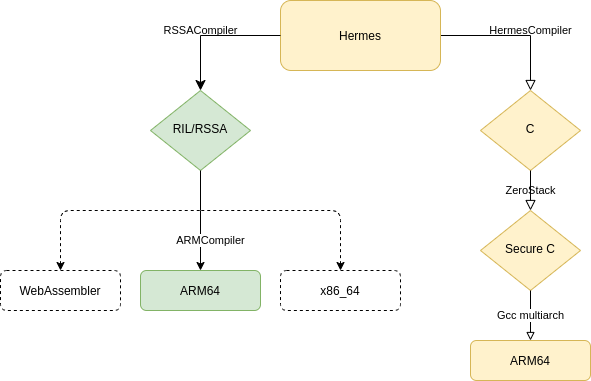
\includegraphics[scale=0.57]{Graphics/compilationProcess.png}
  \caption{Visualization of the project}
  \label{fig:compilationProcess}
\end{figure}

There are a few problems with Hermes in its current implementation, where Hermes programs are translated to C by the program \emph{hc} and then to assembly code with the GNU Compiler Collection (gcc).
We do not have full control over everything that happens in the gcc compiler and gcc does not prevent side-channel attacks, such as information leakage and timing attacks\cite{Simon2018}.
One can use zerostack\cite{Github.zerostack} to zero out the stack and registers of sensitive functions, but this process is very cumbersome and has not yet been thoroughly tested. 
Protection against side-channel attacks would be much easier to enforce with a compilation directly to assembly language, which is the primary focus of this Master thesis.
When we are able to compile directly from Hermes to assembly it will allow us to modify the translation to ensure protection and make it much easier to extend the implementation to other target assembly languages such as WebAssembly or x86\_64.
We make use of the Reversible Single Static Assignment (RSSA) representation from \cite{10.1007/978-3-319-41579-6_16}, which describes how to combine Single Static Assignment (SSA) with Reversible Intermediate Language (RIL) to obtain RSSA.
Furthermore we implement the lightweight cryptography algorithm Twofish in Hermes based on the implementation from the original authors of the algorithm \cite{GIT2F}. We use benchmarks to argue for the correctness of both implementations.




%\input{Sections/1-Introduction/Related_Works.tex}
\section{Outline}
This Master thesis is organized in the following way:
\begin{itemize}
  \item \textbf{Chapter 2} leads off with an introduction to reversibility, side-channel vulnerabilities, the ARM architecture and RSSA.
  \item \textbf{Chapter 3} then analyzes how to compile from Hermes to ARM whilst mitigating side-channels and goes over the parts of ARM we need for the translation.
  \item \textbf{Chapter 4} covers the actual compilation i.e. what steps are taken and how does the program change from source code to intermediate representation to assembly code.
  \item \textbf{Chapter 5} concerns the symmetric encryption algorithm Twofish and my Hermes implementation of it.
  \item \textbf{Chapter 6} is about benchmarks and testing.
  \item \textbf{Chapter 7} is a discussion of the results
  \item In \textbf{Chapter 8} I present my conclusions and ideas for future work.
\end{itemize}
In the appendix I have provided the full implementation of both the ARM compiler and the Twofish implementation in Hermes.


% Baggrund om reversible computing og twofish algoritmen (referer til michaels artikel om reversibel symmetrisk krypto)
\chapter{Background}
\label{chapt - Reversible-computing}
% Skal bruge: Principles of a reversible programming language - Tetsuo, holger bock, robert gluck
%             Partial evaluation of the reversible language Janus - Torben M.
%             Encryption and reversible computations - dominik taborsky, Ken F.L, Michael
%             Reversible computation and reversible PL - Tetsuo
%             TODO: A reversible programming language and its invertible self-interpreter - Yokoyama, robert gluck
%             TODO: Hermes: A reversible language for writing encryption algorithms - Torben MogensenReversible computing is an interesting paradigm with regards to security. In reversible computing one writes programs in reversible programming languages such as Janus [3].
From the early 1960s up until around 2012 we've seen roughly a doubling of transistors in a dense integrated circuit every two years. The limitations associated with increasing computing power seems to be overheating problems. To combat the issue of overheating, research of the programming paradigm Reversible programming started in the early 1970s.

Rolf Landaur, one of the first to talk about reversible programming, argues in\cite{Irreversibility_paper} that any irreversible operation must result in some kind of heat dissipation and that, theoretically, with reversible operations, if operation A pushes the machine from an original state into some new state, then operation A$^{-1}$ could use the existing energy in the system to push it back to the original state.
Such a machine has not yet been invented, but reversible programming has other interesting properties.
As discussed in Section~\ref{chapt - Reversible-computing}, it can serve as protection against side-channel attacks and is also an interesting field to study to better understand quantum computing.

% Landaur embedding is embedding functions inside a larger function that we can then uncall
% Allows for irreversibility but makes the computer more of a lookup table than an actual computer
% We get around this by only allowing logically reversible computations

% Bennet embedding is what we want to use?

\section{Embeddings and heat dissipation}
Another motivation for researching reversible computing is heat dissipation; current transitor-based computing devices dissipate energy as heat and cooling of computational devices has become the main focus for the semiconductor industry \cite{semiconductors_valley}. In 1961 R. Landaur suggested reversible computing could be a way to minimize energy dissipation from a system \cite{Irreversibility_paper}.
Similar to how kinetic and potential energy work, computing a result would put the machine in a state with some energy that would enable it to invert the computation.
Landaur also proposed a way to make irreversible programs reversible. We call this the Landaur embedding.
%Most languages are not reversible, because they throw away information about the computers history, making it ambigious to find the predecessor state. 

%Logic reversibility implies that information is conserved and most languages are not backwards deterministic because some of their operations are logically irreversible and throw away information about the computers history, making it ambiguous to find the predecessor state.
%Embeddings are a way to make an irreversible computer reversible.

\subsection{Landaur embedding}
What Landaur saw was that any logically irreversible program could be transformed into a reversible one by wrapping it in a larger program with extra parameters that could hold any information needed for reversability. He proposed that the computer could have an extra tape where it would save all of its computation history. That way it would know how to run in reverse. But the size of saving this computation history is proportional to the execution time of the program, which is problematic.
Based on the idea that computation is cheap and erasure of data is expensive, Landaur's Embedding is not very efficient since it merely postpones the inevitable erasure of information when the tape needs to be cleared before the next computation.
Landaur demonstrated that whenever a computer throws away information about its previous state it results in a heat dissipation of $kT ln 2$ for each bit of information lost.
\subsection{Bennett embedding}
In 1973 C.H. Bennett came up with a new embedding that would turn out to be much more useful\cite{Bennett1973LogicalRO}.
The idea is that the machine can use the inverse of its transition function to carry out the entire computation backwards, completely resetting the history tape to its original blank state by computation. One only needs to copy over the output once it has been calculated before starting the cleanup. This way the data is reset through computation instead of erasure, which in theory should be much cheaper.
It uses three tapes: one for the forwards/backwards calculation, one for computation history and a third for copying over the output. 
In theory, this reduces the energy dissipated by roughly a factor ten.

\section{Reversibility in Hermes}
% We do not overwrite data in Hermes until we have set it back to 0 at the end of the function?
Hermes is a reversible programming language designed for encryption algorithms. It offers forwards determinism as well as backwards determinism its calculations, meaning that nomatter if it executes forwards or backwards,  there is only one possible state that the machine can transition to nomatter what state it is currently in.
This results in a one-to-one relationship between input and output states that is achieved through reversible updates, swaps and so on.
% Hermes uses pass-by-reference, so no global variables.
Hermes and its predecessor Janus uses pass-by-reference, which is where every argument passed to a function is a direct reference to the variable.
This imposes certain restrictions on parameter passing: there has to be the same amount of parameters for a call / uncall of a function as these are implicitly both the input and output of a function.
There can be no global variables and no variable can be passed to a function multiple times e.g. \emph{foo(x, x, y)}.
Furthermore, an alias on both sides of an update such as \textbf{x += x / y} can break reversibility.

\subsection{Reversible crypto}
% TODO: Something about reversible crypto (twofish) that uses the draw io. Maybe also talk about how fitting hermes is as a language of implementation for hermes. We're using twofish to show how useful Hermes is for crypto algorithms. GFMult is a reversible function and it is used in RSA as well, so we are doing the groundwork for further implementations. Talk about lifting scheme.


% Show control flows
\subsection{Control flows}
Unlike most other programming languages (including Janus), Hermes does not have branching. It has two special types of if-statements being the conditional update and conditional swap which are shown in listing \ref{listing:conditionals_hms}. These conditionals only allow for one line of code to be executed, i.e. the swap or the update, and have a constant execution time. This is because they are constructed in such a way that the code of the conditional is always evaluated but only takes effect or gets executed if the condition is true.
\lstinputlisting[label=listing:conditionals_hms, caption=Conditionals in Hermes, language=Hermes, frame=single] {"Listings/conditionals_in_hermes.hms"}
Conditionals work on integers, which with the help of a logical AND, allows the update to only update in cases where the conditional is non-zero, i.e. true. As seen from listing ~\ref{listing:conditionals_c}, the conditional \textbf{-(0 != a < 2)} evaluates to 0 or -1, which as a signed bit-representation is all bits set to ones, meaning that whatever you AND will remain in the result i.e.
\begin{equation*}
  1111 \& 1011 = 1011
\end{equation*}
This makes the update take effect. Had the conditional evaluated 0, the result of the AND operation would have all its bits set to 0, which would have turned the expression into \textbf{x += 0}.
Swap is done with three XOR operations, which ensures reversability and does not introduce any extra temporary variables.
\lstinputlisting[label=listing:conditionals_c, caption=Conditionals translated to C, language=C, frame=single] {"Listings/conditionals_in_c.c"}

%\begin{figure}
%    \centering
%    \begin{minipage}{0.35\textwidth}
%        \centering
%        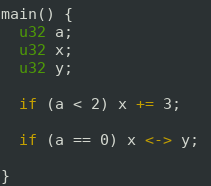
\includegraphics[width=0.9\textwidth]{conditionals_hms.png}
%        \caption{Conditionals in Hermes}
%    \end{minipage}\hfill
%    \begin{minipage}{0.60\textwidth}
%        \centering
%        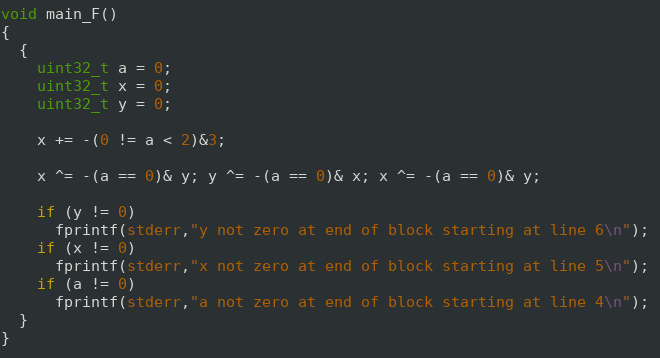
\includegraphics[width=0.9\textwidth]{conditionals_c.png}
%        \caption{Conditionals translated to C}
%        \label{fig:conditionals_c}
%    \end{minipage}
%\end{figure}

% Hermes has const arrays now
\subsection{Constants}
Hermes allows for constant values to be declared. These are not required to be 0 at the end of a function and are initialized with a value other than 0. However, it was only singleton values that were allowed to use the const keyword so I added the ability to specify constant arrays of varying sizes. This was done by adding an entry for it in the AST, the Compiler and the typesystem.
%(* TODO: I also added out of bounds checks *)

Being able to define const arrays is very useful for algorithms such as Twofish that have large 16x16 arrays. In the past, populating large arrays was done through a call to a function that would add values to all the entries of the array. Now it can be done directly in the function that uses it.


\section{Side-channel Vulnerabilities}
Executing a computation on an electronic device consumes time and power, radiates an electromagnetic field, dissipates heat and even makes some noise\cite{Gnad_Krautter_Tahoori_2019}. 
Side-channel attacks aim to take advantage of these leakages, by measuring these physically observable phenomenons; instead of perceiving the cryptographic primitive as a software black box (some transformation that, given some secret parameter, turns some input into output), these new types of attacks target the \emph{environment} such as the process, the processor, the RAM etc. instead of the actual algorithm.

If an adversary is able to extract bits of knowledge about the environment through analysis of running time, power consumption, electromagnetic radiation etc., she may be able to recover the secret parameters involved in the computation.



\label{chapt - Side-channel}
\subsection{Classifying attacks}
Attacks are often classified along two axes falling into one of four categories: \cite{FX2010}.

\begin{itemize}
  \item \textbf{Hardware tampering}
    \begin{itemize}
      \item[1.] Invasive - Attacks which try to read the actual data either by intercepting or directly reading data. An example of this could be to connect a wire onto the data bus and view the data transfers or doing some sort of memory inspection.
      \item[2.] Non-invasive - Attacks which do not read the actual data, but exploits externally available information. External information can be observations on running time, power consumption and such.
    \end{itemize}
  \item \textbf{System tampering}
    \begin{itemize}
      \item[3.] Active - Attacks that tries to change the behaviour of some function on the device, such as introducing a fault in the computation to cause a leak of information, or cold-booting the device to perform memory dumps \cite{Halderman2008LestKeys}.
      \item[4.] Passive - Attacks that only observes a devices behaviour, without affecting it. No signs of compromise or failure.
    \end{itemize}
\end{itemize}

Figure \ref{fig:sca_classification} visualizes these classifications with hardware tampering along the x axis and system tampering along the y axis.
The safety that Hermes intends to provide is against timing attacks and information leakage which includes cold boot attacks.
Timing attacks are non-invasive and passive as the attacker only observes the running time of the process.
Cold boot attacks are active attacks as they perform memory dumps, but can be either invasive or non-invasive exemplified in \cite{Halderman2008LestKeys} where, in one attack, researchers freeze the chip thereby tampering with the hardware.

\begin{figure}[htp]
  \resizebox{0.9\columnwidth}{!}{%
      \begin{tikzpicture}
        \draw [thick] (0,5) node (yaxis) [above] {Active}
          |- (0,-5) node (yaxis) [below] {Passive}
          |- (5,0) node (xaxis) [right] {Invasive}
          |- (-5,0) node (xaxis) [left] {Non-invasive};
        \node[draw, fill=green] at (-4,4) {Cold Boot Attack};
        \node[draw, fill=green] at (4,4) {Cold Boot Attack};
        \node[draw, fill=red] at (-4,-3) {Power analysis};
        \node[draw, fill=green] at (-4,-4) {Timing Attack};
        \node[draw, fill=red] at (4,3) {Row hammer};
        \node[draw, fill=red] at (4,2) {RAMBleed};
        % Legend
        \matrix [draw, below left] at (6,-3.5) {
          \node [fill=green] {Protection\ \ \ \ \ \ \ }; \\
          \node [fill=red] {No Protection}; \\
        }; 
      \end{tikzpicture}%
  }
  \caption{Some side-channel attacks and their classifications} 
  \label{fig:sca_classification}
\end{figure}

Side-channels attacks have been gaining a lot of attention recently by device manufactorers. Especially the non-invasive, passive attacks which are hard to spot and can generally be performed using relatively cheap equipment.

% 2-3 sider
\section{Intermediate representations}
\label{section - RIL}
\subsection{RIL}
RIL stands for Reversible Intermediate Language.
Intermediate languages have been commonly used by compilers since the 1970s.
An intermediate language serves as a common parent-language that, through further compilation, compiles to multiple languages.
It is so to say an \emph{intermediate} result that is never meant to be run, but has some useful features which could allow for optimizations of various kinds.
It often reduces the number of lines of code as well as making it easier to extend, since the first half of the compilation is given, implementing a new end target language requires only half the work.
Thus instead of writing a compiler from $A$ to $B,C,D,E$ we write a compiler for $A$ to intermediate language $I$ and then we use this common ancestor to compile to $B, C, D$ and $E$.
\subsubsection{Entry/Exit points}
A RIL program consists of an unordered set of basic blocks, each defined by an entry point followed by either updates and exchanges or a single subroutine call and is terminated by an exit point\cite{10.1007/978-3-319-41579-6_16}. \\
An entry point has one of the forms:
\begin{verbatim}
l <-        where l is a label,
l1;l2 <- c  where c is a condition and l1 and l2 are labels, or
begin l     where l is a label.
\end{verbatim}
An exit point has one of the forms:
\begin{verbatim}
-> exit     where l is a label,
c -> l1;l2  where c is a condition and l1 and l2 are labels, or
end l       where l is a label.
\end{verbatim}

Each label is unique to the program, i.e. it should occur exactly once in an entry point and once in an exit point.
Furthermore, any label that occurs in an entry point, must also occur in an exit point.
Conditions consists of a left-value, an operator and a right-value.
A left-value can either be a variable such as $x$ or a memory location $M[x]$.
A right-value is either a left-value or a signed constant, and the operator is either ``\lstinline{==, !=, <, <=, >, >=}`` or ``\lstinline{&}``.

\subsubsection{Updates and exchanges}
Updates and exchanges happen inside of the basic blocks that are the RIL program.
Updates consists of a left-value, an update operator, two right-values and an infix arithmetic operation. \\
Left- and right-values have already been introduced. Update operators are ``\lstinline{+=, -=}`` and ``\lstinline{^=}`` and the infix operations are ``\lstinline{+, -, ^, &, |, >>}`` and ``\lstinline{<<}``. It is common to write $x += y$ as a shorthand for $x += y + 0$ as this makes it more readable. \\
An example looks like:
\begin{verbatim}
x += y - 2
\end{verbatim}
Exchanges of variables are of the form
\begin{verbatim}
L1 <-> L2
\end{verbatim}
where $L1$ and $L2$ are left-values.
To ensure reversibility certain restrictions apply:
updates cannot have the same variable or memory access on the left and right side of the update operator and exchanges cannot have the same variable on both sides of the exchange.

\subsubsection{Jumps}
In RIL, the entry and exit points of \emph{main} constitutes the entry and exit points of the entire program. Conditional jumps such as \lstinline{c -> l1;l2} should be read as: \\
\lstinline{if c is true, jump to l1 else jump to l2}. \\
\lstinline{-> exit} is an example of an unconditional jump that will always be executed.

It is important to understand how these entry and exit points are different from standard assembly language jumps/labels.
In most assembly languages, there are certain labels that can be jumped to.
A label could be the beginning of a function, a loop or an if-statement that has two different outcomes.
Because RIL is reversible, there are no seperation between jumps and labels.
All entry points become exit points when reversed and vice-versa.


\subsection{SSA}
% Husk at referer til SSA afsnit i bogen SML compiler
SSA form, which stands for Static Single Assignment form is also a type of intermediate language and is used in compilers such as Java's LLVM compiler\cite{llvm_memory_SSA}.

A compiler can utilize \emph{def-use chains}, which is a data structure with pointers, to quickly jump between definition sites and use sites of variables.
SSA form improves on this idea as a variable with N uses and M definitions will normally take space and time proportional to $N \times M$ for def-use chains, whereas the size of SSA form for most programs will be linear in the size of the original program.
In SSA form, each variable has only one definition in the program text making the \emph{def-use chains} trivial.
SSA form makes it easier to do data-flow analysis such as common-subexpression elimination, value numbering, register allocation and so on.
SSA uses $\phi$-nodes when two variables with the same name are in scope and the compiler needs to know which one it should use.
This happens at so-called join points, which are points that can be reached by two different paths in the code.

Converting to SSA form is a three-step process: first we look at each \emph{definition} of a variable and add an index to it.
Second, we add $\phi$-nodes where it is needed.
Lastly we add indices to variable uses. \\
The article \cite{10.1007/978-3-319-41579-6_16} gives the following example:
\begin{lstlisting}
begin
    x := 0
loop:
    x := x + 1
    if x < 10 then loop else exit
exit:
    x := x + 3
end
\end{lstlisting}
Here we have a loop on $x$ where we add one every iteration until $x$ equals ten.
When we leave the loop, we add another three to $x$.
Translating this to SSA form, we first need to add indices to \emph{definitions}.
\begin{lstlisting}[mathescape=true]
begin
    $x_1$ := 0
loop:
    $x_2$ := x + 1
    if x < 10 then loop else exit
exit:
    $x_3$ := x + 3
end
\end{lstlisting}
Then we add $\phi$-nodes based on join points.
\begin{lstlisting}[mathescape=true]
begin
    $x_1$ := 0
loop:
    $x_4$ := $\phi(x_1, x_2)$
    $x_2$ := x + 1
    if x < 10 then loop else exit
exit:
    $x_3$ := x + 3
end
\end{lstlisting}
And lastly, we add indices to the variable uses.
\begin{lstlisting}[mathescape=true]
begin
    $x_1$ := 0
loop:
    $x_4$ := $\phi(x_1, x_2)$
    $x_2$ := $x_4$ + 1
    if $x_2$ < 10 then loop else exit
exit:
    $x_3$ := $x_2$ + 3
end
\end{lstlisting}
This completes the transformation to SSA form. The definitions and uses of variables are now trivial, making analysis easier.

\subsection{Combing RIL and SSA to RSSA}
The goal is to combine RIL and SSA to Reversible Static Single Assignment (RSSA) form, that will help with program analysis, like tackling the problem of register allocation for reversible languages.

Say we have a C-like program with a for-loop that adds five to $x$ three times:
\begin{lstlisting}
int plus5 (uint_32 x) {
  for (int i = 0; i < 3; i++) {
    x += 5;
  }
  return x;
}
\end{lstlisting}
In RIL this corresponds to:
\begin{lstlisting}[mathescape=true]
begin plus5(x)
i += 0
-> entry
entry; loop <- i == 0
x += 5
i += 1
i < 3 -> loop; exit
exit <-
end plus5(x)
\end{lstlisting}
Keep in mind that \lstinline{entry; loop <- i == 0} is the conditional entry point, meaning that if \lstinline{i == 0}, we are entering from entry, otherwise from loop. In the same fashion, line 7 is a conditional exit point.
From here, we add indices to the definition sites.
\begin{lstlisting}[mathescape=true]
begin plus5($x_n$)
$i_0$ := 0
-> entry
entry; loop <- i == 0
$x_2$ := x + 5
$i_1$ := i + 1
i < 3 -> loop; exit
exit <-
end plus5($x_2$)
\end{lstlisting}
In the second step we add $\phi$-nodes.
\begin{lstlisting}[mathescape=true]
begin plus5($x_n$)
$i_0$ := 0
-> entry
entry; loop <- i == 0
$i_3$ := $\phi(i_0, i_1)$
$x_4$ := $\phi(x_n, x_2)$
$x_2$ := x + 5
$i_1$ := i + 1
i < 3 -> loop; exit
exit <-
end plus5($x_2$)
\end{lstlisting}
In the third step we add indices to variable uses to obtain a representation on RSSA form.
\begin{lstlisting}[mathescape=true]
begin plus5($x_n$)
$i_0$ := 0
-> entry
entry; loop <- $i_1$ == 0
$i_3$ := $\phi(i_0, i_1)$
$x_4$ := $\phi(x_n, x_2)$
$x_2$ := $x_4$ + 5
$i_1$ := $i_3$ + 1
$i_1$ < 3 -> loop; exit
exit <-
end plus5($x_2$)
\end{lstlisting}

\section{Our target assembly language: ARM64}
ARM64 or AArch64 is a family of reduced instruction set computing (RISC) architectures developed by Arm Holdings.
It is currently the most widely used instruction set architecture with more than 100 billion ARM processors produced as of 2017\cite{ARM_sales}. 
ARM is used in many applications, such as Raspberry Pis, self driving cars, phones, tablets etc. Apple, who has been using ARM in their iPhones and iPads recently announced they will be switching from Intel's x86\_64 to ARM64 on their MacBooks from 2020 and onwards\cite{ARM_cpus_2020}.

\subsection{ARM64 vs x86\_64}
% Addressing modes such as load unsigned byte
% Segment registers (CS: code segment, DS: data segment, SS: stack segment, ES: extra segment, FS, GS)
% x86 has variable-length instructions, while ARM is always 32 bit.
% Macro instructions such as ...
% Thumb modes for ARM ...
% CITE [http://www.informit.com/articles/article.aspx?p=1620207&seqNum=3]
Because ARM has a reduced instruction set, it is generally cheaper, less power consuming and dissipates less heat than complex instruction set computing (CISC) architectures such as x86, designed by Intel in the early 80s. This makes it a really great choice for smartphones, laptops and IOT devices.
Intel's x86 has a lot of legacy aspects such as addressing modes and segment registers that are rarely used as well as macro instructions, which can contain several instructions in one and take more work to decode. As a result of this, the ARM pipelines are generally much shorter ranging from 3 to 8 stages compared to that of x86's 14 to 32 stages.  
x86 has variable-length instruction support, whereas the ARM instruction decoder always takes a 32-bit word and just needs to test a few bits to know where to dispatch the instruction. The x86 decoder needs to read the bits in sequence, find breaks between instructions, and so on.  
x86 processors are generally seen as more powerful and a better choice for projects that require complex displays such as gaming or animation, but also require a more power and a heat sink i.e. somewhere to dump their heat dissipation. A high-end Intel i7 processor can consume as much as 130W of power, whereas ARM cores typical power consumption is approximately 5W.
ARM64 is a natural choice for Hermes since our focus is on smaller devices.



\chapter{Problem analysis}
%Afsnit 3 analyserer vi problemet (oversættelsen fra Hermes uden sidekanaler til ARM).
%Hvordan gør vi det egentlig, hvad skal vi være opmærksom på:
%Værktøjer vi bruger, hvorfor bruger vi dem, hvad skal vi gøre for at de kan bruges.
%Når afsnit 3 er færdig, så ved læseren hvad man skal gøre.
In our compilation from Hermes to ARM64 using Moscow ML\footnote{Moscow ML is a functional programming language widely used for teaching and research. More can be found at \url{http://www.itu.dk/~sestoft/mosml.html}}, we need to be aware of several things.

We are skipping some steps, as the current implementation is from Hermes to C and then to ARM.
But by skipping these steps, we have an easier time analyzing and optimizing. The question is how do we do it and what do we need to consider?

\section{Grammar}
In Figure \ref{fig:hermes_grammar} the Hermes grammar is presented.
A Hermes Program consists of one or more Hermes Procedures each with an \bf{id}, a potentially empty list of declarations (function parameters) and a Hermes Block statement consisting of zero or more Hermes Stmts.
One of these Procedures must have the \bf{id} \emph{main} and take no arguments. This is the procedure that is first called when the program is executed.
Every procedure has to have exactly one Block statement. A Block is a special statement corresponding to a function body, consisting of a list of variable declarations followed by a list of Hermes Stmts.
Variable declarations (\emph{Decls1}) can be either variables, dynamic arrays or constants. Constants and constant arrays are public types are therefore not required to be zero at the end of a function. It is the responsibility of the programmer to make sure that sensitive information gets stored in the right variables.
Prior to this thesis Hermes only allowed constant declarations to be variables, but this has been extended allow constant matrix declarations as well.
A ConstArrayDecl in the abstract syntax tree has the type \bf{string * string * string list * typ * pos} which corresponds to name, size, elements, type and position.
\begin{figure}[htp]
\centering
\begin{tabular}{>{$}l<{$}>{$}r<{$}>{$}l<{$}}
    Program   & \rightarrow & Procedure^+ \\[7pt]
    Procedure & \rightarrow & \textbf{id} \; ( \; Decls2^? \; ) \; Stmt \\[7pt]
    Stmt      & \rightarrow &; \\
              & |           & Lval \; \textbf{update} \; Exp \;; \\
              & |           & Lval\text{++} \;; \\
              & |           & Lval\text{- -} \;; \\
              & |           & \texttt{if} \; ( \; Exp \; ) \; Lval \; \textbf{update} \; Exp \;; \\
              & |           & Lval \; \text{<->} \; Lval \;; \\
              & |           & \texttt{if} \; ( \; Exp \; ) \; Lval \; \text{<->} \; Exp \;; \\
              & |           & \texttt{for} \; ( \; \textbf{id} = Exp \; ; \; Exp \; ) \; Stmt  \;; \\
              & |           & \texttt{assert} \; ( \; Exp \; ) \;; \\
              & |           & \texttt{call} \; \textbf{id} \; ( \; Lvals \; ) \;; \\
              & |           & \texttt{uncall} \; \textbf{id} \; ( \; Lvals \; ) \;; \\
              & |           & \texttt{printf} \; ( \; \textbf{stringConst} \; , \; Lvals \; ) \;; \\
              & |           & \texttt{scanf} \; ( \; \textbf{stringConst} \; , \; Lvals \; ) \;; \\
              & |           & \{ \; Decls1 \; Stmt^* \; \} \\[7pt]
    Exp       & \rightarrow & Lval \\
              & |           & \textbf{numConst} \; \\
              & |           & Exp \; \textbf{binOp} \; Exp \\
              & |           & \textbf{unOp} \; Exp \\
              & |           & ( \; Exp \; ) \; \\[7pt]
    Lval      & \rightarrow & \textbf{id}\\
              & |           & \textbf{id} \; [ \; Exp \; ] \\[7pt]
    Lvals     & \rightarrow & Lval \\
              & |           & Lval \; , \; Lvals \\[7pt]
    VarSpec   & \rightarrow & \textbf{id}\\
              & |           & \textbf{id} \; [ \; \textbf{numConst} \; ] \\[7pt]
    VarSpecs  & \rightarrow & VarSpec \\
              & |           & VarSpec \; , \; VarSpecs \\[7pt]
    Decls1    & \rightarrow & \\
              & |           & \textbf{type} \; Varspecs \; ; \; Decls1\\
              & |           & \texttt{const}\;\textbf{type}\;\textbf{id}\;=\textbf{numConst}\;;\;Decls1\;\\[7pt]
    Decls2    & \rightarrow & \textbf{type} \; VarSpec \\
              & |           &  \textbf{type} \; VarSpec \; , \; Decls2

\end{tabular}
\caption{Grammar of Hermes.}
\label{fig: grammar}
\end{figure}



\clearpage
\newpage

\section{Intermediate representations}
When compiling Hermes to RSSA, we use the procedure introduced in Section~\ref{section - RIL}.
We can do this in two iterations: first we translate to RIL, and then we translate to RSSA.
The reason for doing it in two steps is to postpone the problem of register allocation, and keep the two problems seperated.
We will be creating an abstract syntax tree that RIL and RSSA will share.
As seen in Figure~\ref{fig:RIL vs RSSA}, the main difference between the two representations is the subscript index on the left-values.
% TODO: omskriv til egen tabel. Det ser alt for grynet ud med det billede der.
\begin{figure}[htp]
  \begin{center}
    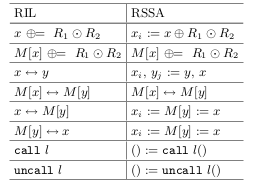
\includegraphics[width=0.6\textwidth]{RIL_RSSA_syntax.png}
  \end{center}
  \caption[caption]{RIL and RSSA syntax from\cite{10.1007/978-3-319-41579-6_16}.}
  \label{fig:RIL vs RSSA}
\end{figure} \\
Variables that are going to have an index can be represented in SML as a tuple of a string variable name and an integer option index. The integer option can be NONE in the first iteration to RIL, and SOME int in the second iteration to RSSA. This makes it easy to seperate the two tasks and handle the indexing once the program has already been transformed to RIL.

Table~\ref{table:translation} shows the correlation between Hermes statements and RSSA statements. Keep in mind that block, printf, scanf and assertion statements do not result in anything as they are only for debugging Hermes.
\begin{table}[htp]
  \begin{tabular}{| a | b |}
    \hline
    \rowcolor{LightCyan}
    \mc{1}{Hermes}      & \mc{1}{RSSA}                  \\ \hline
    Hermes.Skip         & RSSA.Skip                     \\
    Hermes.Update       & RSSA.Assign / RSSA.MemUpdate  \\
    Hermes.CondUpdate   & RSSA.If                       \\
    Hermes.Inc          & RSSA.Assign / RSSA.MemUpdate  \\
    Hermes.Dec          & RSSA.Assign / RSSA.MemUpdate  \\
    Hermes.Swap         & RSSA.AssignSwap / RSSA.MemSwap / RSSA.VarMemSwap \\
    Hermes.CondSwap     & RSSA.If with translated swap inside body \\
    Hermes.For          & RSSA.For  \\
    Hermes.Call         & RSSA.Call \\
    Hermes.Uncall       & RSSA.Uncall \\
    \hline
  \end{tabular}
  \caption{Translation table from Hermes to RSSA.}
  \label{table:translation}
\end{table}

\section{Translation example}
In the following example we will look at a Hermes program that increments a variable and performs an update with addition.
Usually it will be the programmers task to ensure a functions local values are zeroed out before the end of the function. However, to simplify  things we will omit this in the following translation example.

After the parser and the lexer has run, as shown in Listing~\ref{listing:handtranslateHermesInternal}, the internal Hermes representation has the name of the function we are defining ``main``, followed by an empty list of decls i.e. the function parameters.
Then follows the function body as a Block statement with local variable declarations and a list of statements corresponding to the ``\lstinline{++}`` and ``\lstinline{+=}`` statements in Listing~\ref{listing:handtranslateHermes}.

When the RSSA compiler has run, as shown in Listing~\ref{listing:handtranslateRSSAInternal}, the internal Hermes representation has been transformed into an internal RSSA representation containing references to variables and arrays etc.
As there are no RSSA statements for declaring variables, declarations are handled separately as shown in Listing~\ref{listing:handtranslateRSSA}. They are translated to initialization- and finalization-strings in accordance to the RSSA standard from\cite{10.1007/978-3-319-41579-6_16} and inserted by the pretty-printer in case the target language is RIL or RSSA.

When the ARM compiler has run, as shown in Listing~\ref{listing:handtranslateARMInternal}, the internal RSSA representation has been transformed into an internal ARM representation.
As the internal representation of ARM is just a list of instructions, the pretty-printer just prints out the instructions as shown in Listing~\ref{listing:handtranslateARM} and does a little formatting. Rotate left (ROL) becomes rotate right as discussed earlier.

\lstinputlisting[label=listing:handtranslateHermes, caption=Here we see an example of a simple Hermes program that does addition., language=Hermes, float=tp]{"Listings/handtranslateHermes.hms"}

\lstinputlisting[label=listing:handtranslateHermesInternal, caption=Here we see the Hermes internal representation of Listing~\ref{listing:handtranslateHermes}., language=Hermes, float=tp]{"Listings/handtranslateHermesInternal"}

\lstinputlisting[label=listing:handtranslateRSSAInternal, caption=Here we see the RSSA internal representation of Listing~\ref{listing:handtranslateHermes}., language=Hermes, float=tp]{"Listings/handtranslateRSSAInternal"}


\lstinputlisting[label=listing:handtranslateRSSA, caption=Here we see the pretty-printed version of the RSSA internal representation of Listing~\ref{listing:handtranslateRSSAInternal}., float=tp]{"Listings/handtranslateRSSA"}

\lstinputlisting[label=listing:handtranslateARMInternal, caption=Here we see the ARM internal representation of Listing~\ref{listing:handtranslateHermes}., language=Hermes, float=tp]{"Listings/handtranslateARMInternal"}

\lstinputlisting[label=listing:handtranslateARM, caption=Here we see the pretty-printed version of the ARM internal representation of Listing~\ref{listing:handtranslateARMInternal}., language=Hermes, float=tp]{"Listings/handtranslateARM"}

\clearpage
\newpage

\section{Protection from side-channels}
One of the key parts of our compilation is to protect against side-channel attacks.
Hermes does an excellent job of making sure that no sensitive information will be left in memory after execution, but what about timing attacks?
We know that on some architectures, multiplication and division may not be constant time operations.
The modulo operation can also be vulnerable, as it can be implemented using multiplication and division.
One of the most commonly used techniques for modulo is called Barrett Reduction where the general idea is
\begin{equation*}
  X \text{ mod } Y \equiv X - \lfloor{ X / Y }\rfloor Y
\end{equation*}
Here X is divided by Y, floored, and then multiplied with Y. The resulting value is the closest multiple of Y to X. That value is then subtracted from X to give the modulo. 
Fortunately it seems ARM architectures beginning with ARM9E have constant time multiplication and division\cite{bearssl}.
It is still something to keep in mind, however, should we wish to extend Hermes with another target assembly language in the future.

\section{Logical vs physical registers}
The ARM code that is produced by our compiler uses unbounded many abstract logical registers instead of actual physical registers.
It would require a register renaming before the code would actually be able to run on a device.
Register renaming is a technique that is used by high-performance processors to eliminate false data dependencies that can arise from the reuse of registers by successive instructions that do not have any real data dependencies between them.
The elimination of these false data dependencies can result in more instruction-level parallelism in a program, which can be exploited by techniques such as superscalar and out-of-order execution for better performance.
Register renaming or register allocation requires the creation of an inteference graph, which holds information about what values are \emph{simultaneously alive}. The graph is then colored using as few colors as possible. An example is shown in Figure~\ref{fig:interferencegraph} where we see that the same register could hold values a and b as they are not alive at the same time.

\begin{figure}[tp]
  \centering
  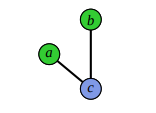
\includegraphics[scale=0.5]{Graphics/interferencegraph.png}
  \caption{An example of a coloured interference graph taken from\cite{ITU_liveness}.}
  \label{fig:interferencegraph}
\end{figure}

In case there are too few registers/colours available to colour the interference graph, the excess values are \emph{spilled}, meaning that they are stored in memory instead.



\chapter{Implementation}
\label{chapt - implementation}
Since RIL and RSSA are so similar in their structure, they share an abstract syntax tree in the implementation.
To enable variables to have indices that occur in RSSA but not in RIL, we use a tuple of type \emph{(string * int option)} as internal representation, where the string is the variable name and int option is the variable index (NONE in the RIL representation).
We alias this tuple as a \emph{var\_idx}.
Listing~\ref{listing:newName} shows the var\_idx generator used for the intermediate variables that our compiler needs.
During the second iteration of compilation we add indices to variables.
We do this by maintaining a list of tuples, which we will use for lookups to keep track of the most recently assigned index for a variable is.
It is also worth mentioning that variables in RIL and RSSA are zeroed at the beginning and end of a function. This is handled by the pretty-printer.

\lstinputlisting[label=listing:newName, caption=Here we see the var\_idx generator. It creates a new var\_idx given some input string. It uses a global counter to generate unique values for the second part of the tuple which is the int option., language=mosml] {"Listings/newName.sml"}

% Section about how to compile from the terminal
\section{Compiling from the terminal}
Compilation is done from the terminal.
Running make from the src folder create an executable \emph{hc} that can be used to compile Hermes into both C, RSSA and ARM.
When running \emph{hc} the default target language is C, but it is possible to change this with a flag such as \lstinline{--rssa} or \lstinline{--arm}.
There is a makefile in the hermes\_v4 folder which will do all of this automatically. Listing~\ref{listing:outerMakefile} shows an extract from this Makefile.
\lstinputlisting[label=listing:outerMakefile, caption=The makefile in hermes\_v4 folder has rules to compile to either RSSA or ARM., language=make, float=htp]{"Listings/outerMakefile"}

% 1: show some of the translation rules from Hermes to RIL. Also talk about the strings that are generated (inits, finits).
\section{Compilation from Hermes to RIL}
When we compile a \emph{Hermes.Update} it consists of an update-operator, an lVal that needs to be updated, an update-expression and a position.
Semantically speaking, the purpose of the \emph{Hermes.Update} is to evaluate the update-expression and update the lVal with respect to the update-operator.
% Show Hermes.Update -> RIL Assign
Listing~\ref{listing:compileStatUpdate} shows how to compile a \emph{Hermes.Update} statement: we begin by compiling the update-expression into an intermediate variable of type \lstinline{(string * int option)} that we create with our var\_idx generator. This is done in compileExp on line 3. Then we need to evaluate the lVal expression as it may contain a nested expression inside the index of an array e.g. $M[x+y]$. This is done in compileLval on line 4.
We now have some code that evaluates the update-expression as well as the lVal.
Now all we need to produce is an update which can either be an \emph{RSSA.Assign} or \emph{RSSA.MemUpdate} depending on the type of the lVal.

\lstinputlisting[label=listing:compileStatUpdate, caption=Here we see the part of the RSSA compiler that handles \emph{Hermes.Update}., language=mosml, float=tp] {"Listings/RSSACompilestatUpdate.sml"}

% 2: show some of the translation rules from RIL to RSSA. Talk about the nontrivial parts (environment, lookup function). Maybe mention invertStat and how we reverse the process. 
\section{Compilation from RIL to RSSA}
% Show RIL Assign -> RSSA Assign
Listing~\ref{listing:rssaTransformAssign} shows how an \emph{RSSA.Assign} is compiled from RIL representation to RSSA representation.
Translating RIL to RSSA requires maintaining an environment to keep track of what variables are currently in scope.
Some intermediate results from compileExp already have their indices, while Assigns with user-defined variables need to have their indices calculated.
We can leave $uop$, $r1$, $binop$ and $r2$ untouched, but we may need to update the index from RIL representation. This transformation would look something like \\
\lstinline{x := x uop r1 binop r2} \bf{->} \lstinline{x_5 := x_4 uop r1 binop r2}. \\
We first need to look up the most recent x.
This is done on line 2-3. Then we handle \lstinline{x_ii} on line 4-6 where we create a new index in case the Assign does not already have one.
On line 7 we update the environment with the new \lstinline{x_ii} and then return the updated \emph{RSSA.Assign}.
% Talk about control statements and show for loop
In case of control structures such as loop- and if-statements, most of the information needed is already given to us in \emph{Hermes.For} so we simply have to pass that along.
The body is recursively translated as shown in Listing~\ref{listing:compileStatFor}.
Converting from RIL to RSSA representation is also done recursively as shown in Listing~\ref{listing:rssaTransformFor}.
\lstinputlisting[label=listing:rssaTransformAssign, caption=Converting an \emph{RSSA.Assign} from RIL to RSSA representation is done by adding indices., language=mosml, float=tp] {"Listings/RSSATransformAssign.sml"}
\lstinputlisting[label=listing:compileStatFor, caption=\emph{Hermes.For} is handled recursively., language=mosml, float=tp] {"Listings/RSSACompilestatFor.sml"}
\lstinputlisting[label=listing:rssaTransformFor, caption=converting an \emph{RSSA.For} from RIL to RSSA representation is done by handling the body recursively., language=mosml, float=htp] {"Listings/RSSATransformFor.sml"}

% 3: show some of the translation rules from RSSA to ARM.
%       Interesting:  * abstract register names and registerallocator
%                     * side-channels and times / div (afsnit 3)
%                     * modulo implementation (hopefully not using div/mul/sub) (afsnit 3)
%                     * static array allocation
%                     * call/uncall using store and load operations as well as stack frames.
\section{Compilation from RSSA to ARM64}
For the final part of translation we need to pick what instructions we want to use for translating the different RSSA statements.
To ensure reversability we do not allow instructions such as \emph{LSL} (logical shift left) and \emph{LSR} (logical shift right) as these would throw away bits when shifting them off the end.
Instead we use \emph{ROR} (rotate right) which inserts the bits that are rotated off to the right on the vacated bit positions on the left.
We do not need to worry about only having rotate right available to us, as it can function as a rotate left if we subtract the bits we want to rotate left from $64$ and rotate right instead.
We define \emph{ROL} as a pseudo-instruction as
\begin{equation*}
  ROL(x) == ROR(64-x).
\end{equation*}
% RSSA Assign -> ARM
Listing~\ref{listing:ARMCompilestatAssign.sml} shows the compilation process for \emph{RSSA.Assign} to ARM.
Five out of six values are optional, so the amount of combinations to check for could be $1 \times 2^5 = 32$.
But not all combinations are possible, thus by pattern matching we actually reduce it to 5 different combinations:\\
The first case handles updates with constants \lstinline{xi := const c}.
The second one handles updates with array indexing \lstinline{xi := M[x]}.
The third one handles some of the intermediate results generated from the RSSA compilation step where \lstinline{xi := x}.
The fourth case handles \lstinline{xi := x uop r1}.
The fifth one handles the full \lstinline{xi := x uop r1 binop r2} that were mentioned earlier in Figure~\ref{fig:RIL vs RSSA}.

\lstinputlisting[label=listing:ARMCompilestatAssign.sml, caption=Compiling \emph{RSSA.Assign} is done by pattern matching. This reduces code size., language=mosml, float=htp] {"Listings/ARMCompilestatAssign.sml"}

\section{Logical vs physical registers}
The ARM code that is produced by our compiler uses unbounded many abstract logical registers instead of actual physical registers.
Once a register allocator is added, the code would be able to run on a device.
Register allocation requires the creation of an inteference graph, which holds information about what values are \emph{simultaneously alive}. The graph is then colored using as few colors as possible. An example is shown in Figure~\ref{fig:interferencegraph} where we see that the same register could hold values a and b as they are not alive at the same time.
In case there are too few registers/colours available to colour the interference graph, the register allocator \emph{spills} the excess values to memory by inserting store/load operations.

\begin{figure}[tp]
  \centering
  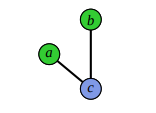
\includegraphics[scale=0.5]{Graphics/interferencegraph.png}
  \caption{An example of a coloured interference graph taken from\cite{ITU_liveness}.}
  \label{fig:interferencegraph}
\end{figure}

%\input{Sections/Grammars/RSSA_grammar.tex}
%\input{Sections/Grammars/ARM_grammar.tex}

% Afsnit om min twofish implementation med referencer til twofish bogen
\chapter{Twofish}
\label{chapt - Twofish}
\section{The algorithm}
In 1972 and 1974, the National Bureau of Standards (now the National Institute of Standards and Technology, or NIST) issued the first public request for an encryption standard. The result was DES\cite{NBS77}, which became widely used and a very successful encryption algorithm at the time. However, due to advances in distributed key search techniques, the key was found to be too short for modern security applications.
Triple-DES emerged as a temporary solution in many high-security applications, such as banking, but was too slow. More fundamentally, the $64$-bit block length shared by DES and most other well-known ciphers opens it up to attacks when large amounts of data are encrypted under the same key.

Twenty years later, in 1997, NIST announced the Advanced Encryption Standard (AES)\cite{NIST97a}. NIST requested comments from the public on the proposed standard, and eventually issued a call for algorithms to satisfy the standard\cite{NIST97b}. NIST made all submissions public and eventually, through a process of public review and comment, chose a new encryption standard to replace DES. Twofish did not win, but made it as one of the five finalists in the 1997 competition.

Figure~\ref{fig:twofish} shows the Twofish algorithm. It is a $16$ byte / $128$-bit block cipher with a variable key length between $128$ and $256$ bits.
The cipher is a $16$-round Feistel network also called a substitute-permute network. It has a bijective function $F$ consisting of four key-dependent $8$-by-$8$-bit S-boxes (Substitution-boxes)\cite{wiki_sbox}, a fixed $4$-by-$4$ MDS (maximum distance separable) matrix over GF($2^8$) (Galois-field), a PHT (pseudo-Hadamard transform), bitwise rotations, and a carefully designed key schedule.
\begin{figure}[tp]
  \centering
  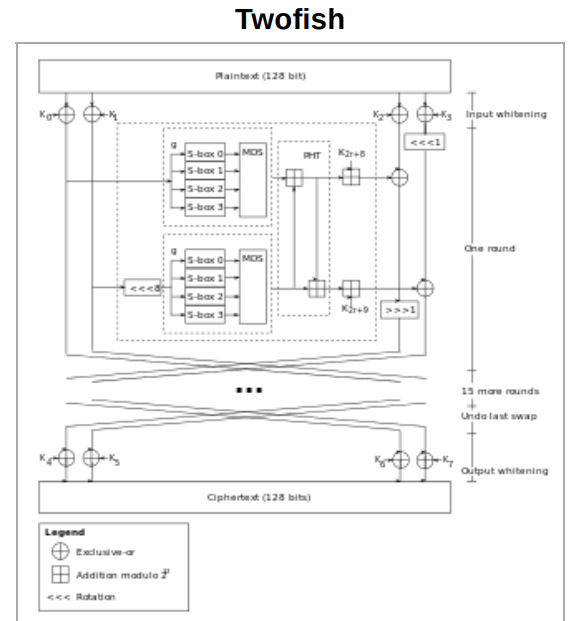
\includegraphics[scale=0.4]{Graphics/twofish.png}
  \caption{The Twofish algorithm}
  \label{fig:twofish}
\end{figure}

\subsection{Feistel Networks}
A Feistel network is a general method of transforming any function (usually called the F function) into a permutation. It was invented by Horst Feistel in 1973.

The fundamental building block of a Feistel network is the $F$ function: a key-dependent mapping of an input string onto an output string. An $F$ function is always non-linear and possibly non-surjective\footnote{A non-surjective F function is one in which not all outputs in the output space can occur.}:

\begin{equation*}
  F : \lbrace 0, 1\rbrace^{n/2} x \lbrace0, 1\rbrace^N -> \lbrace 0, 1\rbrace^{n/2}
\end{equation*}

where $n$ is the block size of the Feistel network, and $F$ is a function taking $n/2$ bits of the block and $N$ bits of a key as input, and producing an output of length $n/2$ bits.
In each round, the ``source block`` is the input to $F$ , and the output of $F$ is XOR'ed with the ``target block``, after which these two blocks swap places for the next round.
The idea here is to take an $F$ function, which may be a weak encryption algorithm when taken by itself, and repeatedly iterate it to create a strong encryption algorithm.
Two rounds of a Feistel network is called a \emph{cycle}.
In one cycle, every bit of the text block has been modified once.

This is in fact very similar to what happens in \emph{discrete wavelet transformation} (DWT), where the technique called a \emph{lifting scheme} was introduced by Wim Sweldens.

\subsection{S-boxes}
An S-box is a table-driven non-linear substitution operation used in most block ciphers.
S-boxes vary in both input size and output size, and can be created either randomly or algorithmically.
S-boxes were first used in Lucifer by Horst Feistel, then DES, and afterwards in most encryption algorithms.
Twofish uses four different, bijective, key-dependent, $8$-by-$8$-bit S-boxes.
These S-boxes are built using two fixed $8$-by-$8$-bit permutations and key material.

\subsection{A small 2-by-2-bit S-box example}
Substitute-permute networks, as the name implies, perform a substitution followed by a permutation.
Two bits can have four different values: ``00``, ``01``, ``10`` and ``11``, so a table could look like this:
\begin{table}[htp]
  \begin{center}
    \label{fig:small_subs_example}
    \begin{tabular}{|l|c|c|c|c|}
      \hline
      input  & 00 & 01 & 10 & 11 \\ \hline
      output & 10 & 00 & 11 & 01 \\ \hline
    \end{tabular}
  \end{center}
\end{table}

If ``10`` enters the table, it becomes substituted to ``11`` and if ``11`` enters it becomes substituted to ``01``.
Given two of these $2$-by-$2$-bit S-boxes, the output would be 2 bits from each, equalling $4$ in total.
The permutation part is switching bits and could look like this:
\begin{table}[htp]
  \begin{center}
    \label{fig:small_permu_example}
    \begin{tabular}{|l|c|c|c|c|c|c|c|c|}
      \hline
      input  & 0  & 1  & 2  & 3  & 4  & 5  & 6  & 7  \\ \hline
      output & 6  & 13 & 15 & 1  & 7  & 12 & 8  & 3  \\ \hline
      input  & 8  & 9  & 10 & 11 & 12 & 13 & 14 & 15 \\ \hline
      output & 2  & 0  & 14 & 10 & 5  & 9  & 11 & 4  \\ \hline
    \end{tabular}
  \end{center}
\end{table}

Given input ``0100``, the first Sbox would have input ``01`` and the second Sbox to have input ``00``.
The output of the first S-box equals ``00`` and the output of the second S-box equals ``10``.
So in decimal, the number $4$ goes through the two S-boxes and comes out as a $2$.
Then it enters the permutation table and becomes $15$ constituting one round of substituting and permuting.
This process is very easy to reverse if the substition table and the permutation table are public, hence Twofish mixes in keys via XOR.
It XORs before the first encryption (input whitening), after each round, and again after the last round (output whitening).
Without the key, the process becomes very hard to reverse.
There is a trade-off of security versus speed; too few rounds makes the encryption breakable whereas too many rounds will make it slow.
Twofish uses $16$ rounds compared to the $10-14$ for AES depending on key size.

\subsection{Maximum Distance Seperable matrices}
An MDS matrix is a linear mapping from $a$ field elements to $b$ field elements. It produces a composite vector of $a + b$ elements with the property that for each non-zero vector there will be atleast $b + 1$ non-zero elements.
What this means is that the ``distance`` (i.e. the number of elements that differ) between two distinct vectors produced by the MDS mapping is atleast $b + 1$.
It is provable that no mapping can have a larger minimum distance between two distinct vectors\cite{TwofishPaper}, hence we call it Maximum Distance Seperable.
Twofish uses a $4$-by-$4$ MDS matrix over GF ($2^8$) called the Reed-Solomon (RS) error-correcting codes.

\subsection{Pseudo-Hadamard transforms}
The $32$-bit pseudo-Hadamard transform (PHT) that Twofish uses is a mixing operation that given two inputs $a$ and $b$, updates the two values as follows:
\begin{equation*}
  a' = a + b\text{ mod }2^{32} \\
\end{equation*}
\begin{equation*}
  b' = a + 2b\text{ mod }2^{32}
\end{equation*}
This is used to mix the two outputs of its \emph{g} function calls.

\subsection{Whitening}
Input/output whitening is done by XOR'ing $128$ bits of subkey, which is not used in any of the rounds, with part of the expanded key before the first round and after the last round. It was shown in 1996 by Rivest\cite{KR96} that whitening made it substantially harder for attackers to do keysearch attacks.

\subsection{Key schedule}
\label{section:key_schedule}
The key schedule is the means by which the key bits are turned into round keys that the cipher can use.  Twofish needs a lot of key material, and has a complicated key schedule. To facilitate analysis, the key schedule uses the same primitives as the round function.

There are two types of keys used for the Twofish algorithm.
It uses a user-supplied global key $M$ of $128$ bits to generate two sets of subkeys $S$ and $K$.
$S$ has two subkeys $S_0$ and $S_1$ which are fixed during the entire encryption and decryption process.
$S_0$ and $S_1$ are used in the S-boxes inside the g function.
The key schedule performs a key expansion to make K, which is a $40$-word expanded key where each word consists of $32$ bits.
$K_0$-$K_7$ are used for input / output whitening whilst the remaining $32$ words are passed to the bijective function F two at a time during the 16 rounds of encryption.
$S$ is generated by finite field multiplication in Galois Field GF$(2^8)$ where the primitive polynomial is $x^8 + x^6 + x^3 + x^2 + 1$.
Finite field multiplication would be implemented in Hermes using Bennett embedding, as the multiplication can sometimes have values that are zero.
Bennett embedding would allow us to save the values until decomputed later.

\section{Reversible Twofish}
\subsection{Reference implementation}
Bruce Schneier, who is a co-author of the algorithm, has a Github repository \cite{Git2F} with two implementations of Twofish: A highly optimized one in C and another one in Python2.7.
I will be focusing on the Python implementation as it is more similar to the Hermes implementation in its structure as well as being easier to read.
Its around 250 lines of code, so not awfully large but not small either. The complexity of the code is low/medium and it is overall pretty straight forward if you know how the algorithm works.

TODO: Snak om lifting scheme + konkluder hvorvidt Hermes er passende som domænespecifikt krypteringssprog

\subsection{encrypt/decrypt}
\subsubsection{Python}
Lets look at the encrypt/decrypt definitions.
\lstinputlisting[label=app:Encrypt Python,caption=encrypt/decrypt in Python, language=Python,frame=single] {"Listings/encrypt.py"}
We see that the only difference between encrypt and decrypt is the order in which they do things.
Encrypt uses the words K[0]-K[3] for input whitening, calls F 16 times with roundnumber r = 0 to 16, and then performs output whitening with the words K[4]-K[7]. Decrypt does the same but in the other direction. 

The parameters for the functions are subkeys K and S as well as a plaintext/ciphertext.
They both call F with five arguments: input words R[0] and R[1], the round number r which is used to select which subkeys to use, and the subkeys K and S.

\subsubsection{Hermes}
My implementation is structurally similar to the Python version. Lets have a look:
\lstinputlisting[label=app:Encrypt Hermes,caption=encrypt in Hermes, language=Hermes,frame=single] {"Listings/encrypt.hms"}
Here we see the same structure; input whitening followed by 16 rounds of encryption followed by output whitening. It has the same logic (calling F and rotating/XOR'ing) as the Python implementation. TODO: It uses Bennetts method of passing along some placeholder variables that can store some intermediate values which we can use to reset the inplace updated variables later with uncall.

\subsection{Galois Field multiplication}
Lorem ipsum..
%TODO: Galois Field multiplication is interesting because

\subsubsection{Python}
\lstinputlisting[label=app:GaloisField Python,caption=Galois Field multiplication in Python, language=Python,frame=single] {"Listings/gfmult.py"}

\subsubsection{Hermes}
%TODO: Det her må ku gøres pænere med flags array
%TODO: Polymult bruger Bennet? Snak om B ikke må være 0. Burde aldrig ske siger michael.
%TODO: GFMult er som sådan en reversibel funktion siger michael og den optræder i RSA. Konkluder evt. noget med at det her er babysteps towards en RSA implementation?
\lstinputlisting[label=app:GaloisField Hermes,caption=Galois Field multiplication in Hermes, language=Hermes,frame=single] {"Listings/gfmult.hms"}


% Kør min implementation af twofish 50 gange imod deres 50 gange
\chapter{Benchmarks}
\label{chapt - Benchmarks}
% Simple eksempler som jeg går i detaljer med
\section{Compilation}
test 

\section{Correctness}
test2

\section{Twofish}
test3



\chapter{Discussion}
\label{chapt - Discussion}
%%Afsnit 3 analyserer vi problemet (oversættelsen fra Hermes uden sidekanaler til ARM).
%Hvordan gør vi det egentlig, hvad skal vi være opmærksom på:
%Værktøjer vi bruger, hvorfor bruger vi dem, hvad skal vi gøre for at de kan bruges.
%Når afsnit 3 er færdig, så ved læseren hvad man skal gøre.
In our compilation from Hermes to ARM64 using Moscow ML\footnote{Moscow ML is a functional programming language widely used for teaching and research. More can be found at \url{http://www.itu.dk/~sestoft/mosml.html}}, we need to be aware of several things.

We are skipping some steps, as the current implementation is from Hermes to C and then to ARM.
But by skipping these steps, we have an easier time analyzing and optimizing. The question is how do we do it and what do we need to consider?

\section{Grammar}
In Figure \ref{fig:hermes_grammar} the Hermes grammar is presented.
A Hermes Program consists of one or more Hermes Procedures each with an \bf{id}, a potentially empty list of declarations (function parameters) and a Hermes Block statement consisting of zero or more Hermes Stmts.
One of these Procedures must have the \bf{id} \emph{main} and take no arguments. This is the procedure that is first called when the program is executed.
Every procedure has to have exactly one Block statement. A Block is a special statement corresponding to a function body, consisting of a list of variable declarations followed by a list of Hermes Stmts.
Variable declarations (\emph{Decls1}) can be either variables, dynamic arrays or constants. Constants and constant arrays are public types are therefore not required to be zero at the end of a function. It is the responsibility of the programmer to make sure that sensitive information gets stored in the right variables.
Prior to this thesis Hermes only allowed constant declarations to be variables, but this has been extended allow constant matrix declarations as well.
A ConstArrayDecl in the abstract syntax tree has the type \bf{string * string * string list * typ * pos} which corresponds to name, size, elements, type and position.
\begin{figure}[htp]
\centering
\begin{tabular}{>{$}l<{$}>{$}r<{$}>{$}l<{$}}
    Program   & \rightarrow & Procedure^+ \\[7pt]
    Procedure & \rightarrow & \textbf{id} \; ( \; Decls2^? \; ) \; Stmt \\[7pt]
    Stmt      & \rightarrow &; \\
              & |           & Lval \; \textbf{update} \; Exp \;; \\
              & |           & Lval\text{++} \;; \\
              & |           & Lval\text{- -} \;; \\
              & |           & \texttt{if} \; ( \; Exp \; ) \; Lval \; \textbf{update} \; Exp \;; \\
              & |           & Lval \; \text{<->} \; Lval \;; \\
              & |           & \texttt{if} \; ( \; Exp \; ) \; Lval \; \text{<->} \; Exp \;; \\
              & |           & \texttt{for} \; ( \; \textbf{id} = Exp \; ; \; Exp \; ) \; Stmt  \;; \\
              & |           & \texttt{assert} \; ( \; Exp \; ) \;; \\
              & |           & \texttt{call} \; \textbf{id} \; ( \; Lvals \; ) \;; \\
              & |           & \texttt{uncall} \; \textbf{id} \; ( \; Lvals \; ) \;; \\
              & |           & \texttt{printf} \; ( \; \textbf{stringConst} \; , \; Lvals \; ) \;; \\
              & |           & \texttt{scanf} \; ( \; \textbf{stringConst} \; , \; Lvals \; ) \;; \\
              & |           & \{ \; Decls1 \; Stmt^* \; \} \\[7pt]
    Exp       & \rightarrow & Lval \\
              & |           & \textbf{numConst} \; \\
              & |           & Exp \; \textbf{binOp} \; Exp \\
              & |           & \textbf{unOp} \; Exp \\
              & |           & ( \; Exp \; ) \; \\[7pt]
    Lval      & \rightarrow & \textbf{id}\\
              & |           & \textbf{id} \; [ \; Exp \; ] \\[7pt]
    Lvals     & \rightarrow & Lval \\
              & |           & Lval \; , \; Lvals \\[7pt]
    VarSpec   & \rightarrow & \textbf{id}\\
              & |           & \textbf{id} \; [ \; \textbf{numConst} \; ] \\[7pt]
    VarSpecs  & \rightarrow & VarSpec \\
              & |           & VarSpec \; , \; VarSpecs \\[7pt]
    Decls1    & \rightarrow & \\
              & |           & \textbf{type} \; Varspecs \; ; \; Decls1\\
              & |           & \texttt{const}\;\textbf{type}\;\textbf{id}\;=\textbf{numConst}\;;\;Decls1\;\\[7pt]
    Decls2    & \rightarrow & \textbf{type} \; VarSpec \\
              & |           &  \textbf{type} \; VarSpec \; , \; Decls2

\end{tabular}
\caption{Grammar of Hermes.}
\label{fig: grammar}
\end{figure}



\clearpage
\newpage

\section{Intermediate representations}
When compiling Hermes to RSSA, we use the procedure introduced in Section~\ref{section - RIL}.
We can do this in two iterations: first we translate to RIL, and then we translate to RSSA.
The reason for doing it in two steps is to postpone the problem of register allocation, and keep the two problems seperated.
We will be creating an abstract syntax tree that RIL and RSSA will share.
As seen in Figure~\ref{fig:RIL vs RSSA}, the main difference between the two representations is the subscript index on the left-values.
% TODO: omskriv til egen tabel. Det ser alt for grynet ud med det billede der.
\begin{figure}[htp]
  \begin{center}
    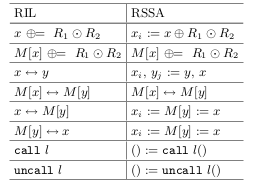
\includegraphics[width=0.6\textwidth]{RIL_RSSA_syntax.png}
  \end{center}
  \caption[caption]{RIL and RSSA syntax from\cite{10.1007/978-3-319-41579-6_16}.}
  \label{fig:RIL vs RSSA}
\end{figure} \\
Variables that are going to have an index can be represented in SML as a tuple of a string variable name and an integer option index. The integer option can be NONE in the first iteration to RIL, and SOME int in the second iteration to RSSA. This makes it easy to seperate the two tasks and handle the indexing once the program has already been transformed to RIL.

Table~\ref{table:translation} shows the correlation between Hermes statements and RSSA statements. Keep in mind that block, printf, scanf and assertion statements do not result in anything as they are only for debugging Hermes.
\begin{table}[htp]
  \begin{tabular}{| a | b |}
    \hline
    \rowcolor{LightCyan}
    \mc{1}{Hermes}      & \mc{1}{RSSA}                  \\ \hline
    Hermes.Skip         & RSSA.Skip                     \\
    Hermes.Update       & RSSA.Assign / RSSA.MemUpdate  \\
    Hermes.CondUpdate   & RSSA.If                       \\
    Hermes.Inc          & RSSA.Assign / RSSA.MemUpdate  \\
    Hermes.Dec          & RSSA.Assign / RSSA.MemUpdate  \\
    Hermes.Swap         & RSSA.AssignSwap / RSSA.MemSwap / RSSA.VarMemSwap \\
    Hermes.CondSwap     & RSSA.If with translated swap inside body \\
    Hermes.For          & RSSA.For  \\
    Hermes.Call         & RSSA.Call \\
    Hermes.Uncall       & RSSA.Uncall \\
    \hline
  \end{tabular}
  \caption{Translation table from Hermes to RSSA.}
  \label{table:translation}
\end{table}

\section{Translation example}
In the following example we will look at a Hermes program that increments a variable and performs an update with addition.
Usually it will be the programmers task to ensure a functions local values are zeroed out before the end of the function. However, to simplify  things we will omit this in the following translation example.

After the parser and the lexer has run, as shown in Listing~\ref{listing:handtranslateHermesInternal}, the internal Hermes representation has the name of the function we are defining ``main``, followed by an empty list of decls i.e. the function parameters.
Then follows the function body as a Block statement with local variable declarations and a list of statements corresponding to the ``\lstinline{++}`` and ``\lstinline{+=}`` statements in Listing~\ref{listing:handtranslateHermes}.

When the RSSA compiler has run, as shown in Listing~\ref{listing:handtranslateRSSAInternal}, the internal Hermes representation has been transformed into an internal RSSA representation containing references to variables and arrays etc.
As there are no RSSA statements for declaring variables, declarations are handled separately as shown in Listing~\ref{listing:handtranslateRSSA}. They are translated to initialization- and finalization-strings in accordance to the RSSA standard from\cite{10.1007/978-3-319-41579-6_16} and inserted by the pretty-printer in case the target language is RIL or RSSA.

When the ARM compiler has run, as shown in Listing~\ref{listing:handtranslateARMInternal}, the internal RSSA representation has been transformed into an internal ARM representation.
As the internal representation of ARM is just a list of instructions, the pretty-printer just prints out the instructions as shown in Listing~\ref{listing:handtranslateARM} and does a little formatting. Rotate left (ROL) becomes rotate right as discussed earlier.

\lstinputlisting[label=listing:handtranslateHermes, caption=Here we see an example of a simple Hermes program that does addition., language=Hermes, float=tp]{"Listings/handtranslateHermes.hms"}

\lstinputlisting[label=listing:handtranslateHermesInternal, caption=Here we see the Hermes internal representation of Listing~\ref{listing:handtranslateHermes}., language=Hermes, float=tp]{"Listings/handtranslateHermesInternal"}

\lstinputlisting[label=listing:handtranslateRSSAInternal, caption=Here we see the RSSA internal representation of Listing~\ref{listing:handtranslateHermes}., language=Hermes, float=tp]{"Listings/handtranslateRSSAInternal"}


\lstinputlisting[label=listing:handtranslateRSSA, caption=Here we see the pretty-printed version of the RSSA internal representation of Listing~\ref{listing:handtranslateRSSAInternal}., float=tp]{"Listings/handtranslateRSSA"}

\lstinputlisting[label=listing:handtranslateARMInternal, caption=Here we see the ARM internal representation of Listing~\ref{listing:handtranslateHermes}., language=Hermes, float=tp]{"Listings/handtranslateARMInternal"}

\lstinputlisting[label=listing:handtranslateARM, caption=Here we see the pretty-printed version of the ARM internal representation of Listing~\ref{listing:handtranslateARMInternal}., language=Hermes, float=tp]{"Listings/handtranslateARM"}

\clearpage
\newpage

\section{Protection from side-channels}
One of the key parts of our compilation is to protect against side-channel attacks.
Hermes does an excellent job of making sure that no sensitive information will be left in memory after execution, but what about timing attacks?
We know that on some architectures, multiplication and division may not be constant time operations.
The modulo operation can also be vulnerable, as it can be implemented using multiplication and division.
One of the most commonly used techniques for modulo is called Barrett Reduction where the general idea is
\begin{equation*}
  X \text{ mod } Y \equiv X - \lfloor{ X / Y }\rfloor Y
\end{equation*}
Here X is divided by Y, floored, and then multiplied with Y. The resulting value is the closest multiple of Y to X. That value is then subtracted from X to give the modulo. 
Fortunately it seems ARM architectures beginning with ARM9E have constant time multiplication and division\cite{bearssl}.
It is still something to keep in mind, however, should we wish to extend Hermes with another target assembly language in the future.

\section{Logical vs physical registers}
The ARM code that is produced by our compiler uses unbounded many abstract logical registers instead of actual physical registers.
It would require a register renaming before the code would actually be able to run on a device.
Register renaming is a technique that is used by high-performance processors to eliminate false data dependencies that can arise from the reuse of registers by successive instructions that do not have any real data dependencies between them.
The elimination of these false data dependencies can result in more instruction-level parallelism in a program, which can be exploited by techniques such as superscalar and out-of-order execution for better performance.
Register renaming or register allocation requires the creation of an inteference graph, which holds information about what values are \emph{simultaneously alive}. The graph is then colored using as few colors as possible. An example is shown in Figure~\ref{fig:interferencegraph} where we see that the same register could hold values a and b as they are not alive at the same time.

\begin{figure}[tp]
  \centering
  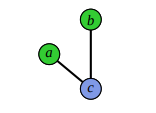
\includegraphics[scale=0.5]{Graphics/interferencegraph.png}
  \caption{An example of a coloured interference graph taken from\cite{ITU_liveness}.}
  \label{fig:interferencegraph}
\end{figure}

In case there are too few registers/colours available to colour the interference graph, the excess values are \emph{spilled}, meaning that they are stored in memory instead.



% Man kunne helt gak skrive noget om kvantecomputere her - nej det går ikke
% Kunne måske også nævne noget om Rust oversættelse\chapter{Conclusion}
\label{chapt - Conclusion}
I've shown that Hermes is well suited to higher complexity encryption algorithms involving lifting schemes and Galois Field multiplications.


Property based testing af Twofish ala det Simon brugte
Biblioteker til GFMult så vi kan komme i mål med RSA og keySched til Twofish


% Til diskussionen kan man nævne Iodine: verifying constant-time execution of hardware artiklen?




% Referencer
\newpage
\bibliographystyle{plain}
\renewcommand\bibname{References}
\bibliography{references}

%SSA afsnit i Modern compiler implementation in ML af Andrew w. Appel


% Appendices
\clearpage
\newpage
\begin{appendices}
\renewcommand*{\lstlistingname}{Appendix}
\chapter{Compilers}
\label{appendix:A}
\section{RSSA Compiler}
\lstinputlisting[label=appendix:RSSACompiler.sml, caption=RSSACompiler in MosML, language=mosml,frame=single] {"Listings/RSSACompiler.sml"}

\newpage
\section{ARM Compiler}
\label{appendix:RC5_Full_Imp}


\chapter{Twofish}
\lstinputlisting[label=:appendix:Twofish.hms, caption=Reversible Twofish in Hermes, language=Hermes, frame=single] {"Listings/twofish.hms"}

\chapter{Tests}
\end{appendices}

\end{document}
